
%|  Name  | TODO | ONGOING | DONE |
%|--------|------|---------|------|
%| Dana   | x    |         |      |
%| Gerd   | x    |         |      |
%| Glenn  | x    |         |      |
%| Jordan | x    |         |      |
%| Luke   | x    |         |      |
%| Matt   |      |         | x    |
%| Neil   | x    |         |      |
%| Scot   | x    |         |  x    |

%\todo[inline]{Owner: Matt -- Priority: High -- Effort: M - Completion: 100\%}
Continuing in the educational tours, we will delve into the intricate details of datatypes, their categories, and how they are represented and managed by the HDF5 library. We will also explore the encoding process of datatypes for disk storage and how the library handles data of different data types in the file.

 Moreover, we will also highlight the remarkable extensibility and customizability of the HDF5 library, which empowers users to define their own datatypes, composite datatypes, and datatype conversion functions. This capability allows for optimizing almost every I/O process step.
\subsection{Datatype life cycle}

Speaking broadly, the datatype life cycle begins at build configuration time with the discovery of platform-specific types, proceeds at run-time during library initialization, and continues with the construction of predefined and user-defined datatypes. In this section, we describe the library infrastructure supporting this process.

\paragraph{Configuration-Time Type Discovery} The HDF5 library checks the size of each built-in C type on the current platform at configuration time. A set of macros with names of the form \texttt{H5\_SIZEOF\_<TYPE>} will be defined in the generated file \texttt{H5pubconf.h}. These macros define an internal assignment operator between numeric types that works regardless of the types' relative sizes, \texttt{H5\_CHECKED\_ASSIGN}.

\paragraph{Predefined Datatypes} The types predefined by the library have standard symbolic names of the form \texttt{H5T\_<arch>\_<base>} where 'arch' is an architecture name, and 'base' is a programming type name formed from a letter for the type class, a number for the precision in bits, and an indication of byte order. For example, \texttt{H5T\_INTEL\_I64BE} is a predefined type for 64-bit big-endian integers on Intel CPUs.

The names through which the predefined types are accessed are defined as macros in \texttt{H5Tpublic.h}. The macro \texttt{H5T\_<TYPE>} evaluates to \texttt{H5OPEN H5T\_<TYPE>\_g}. \texttt{H5OPEN} is a macro that ensures the library is initialized if the type macro was used in a public or user application file. \texttt{H5T\_<TYPE>\_g} is a globally accessible handle ID for the predefined type.

Predefined types' inability to be modified is implemented through the \texttt{state} field of \texttt{H5T\_t}'s shared information. Predefined types are created with their state set to immutable, making them unmodifiable and unable to be closed by the user.

\paragraph{Predefined Datatype Initialization} The H5T package is initialized during phase 2 of H5VL's initialization, as seen in Listing~\ref{lst:vol2-init-table}. An internal diagram of \texttt{H5T\_init} is shown in Figure~\ref{fig:h5t-init-table}.

Predefined types that match the native platform are created first in two steps. In the first step, predefined float datatypes that match the native platform are created and registered in \\ \texttt{H5T\_\_init\_native\_float\_types}. The \texttt{DETECT\_F} macro detects the native platform's floating-point properties, which are used to construct matching datatypes. The datatypes are assigned library handles by \texttt{H5I\_register}. These handles are stored in a set of global variables with names of the form \texttt{H5T\_NATIVE\_<TYPE>\_g}. In the second step, a similar process is carried out for all other native datatypes in \texttt{H5T\_\_init\_native\_internal}, using detected information about the platform's byte order and alignment.

Once the predefined native datatypes are created, they are used to create the predefined non-native datatypes through the macro \texttt{H5T\_INIT\_TYPE}. If the new type to be constructed is based on an existing one, this macro copies the provided base type with \texttt{H5T\_copy} before making size and byte order modifications. If the new type is not based on an existing type, the macro directly allocates space for a new \texttt{H5T\_t} structure and populates it using another macro of the form \texttt{H5T\_INIT\_TYPE\_<TYPE>\_CORE}. In both cases, \texttt{H5T\_INIT\_TYPE} registers the newly created datatype with the library, assigns it a handle through \texttt{H5I\_register}, and makes the handle globally accessible through \texttt{H5T\_<ARCH>\_<BASE>\_g}. A user can then access these handles through macros of the form \texttt{H5T\_<ARCH>\_<BASE>}, as discussed in the previous section. 

In addition to initializing predefined datatypes, \texttt{H5T\_init} also sets up many internal datatype conversion routines through \texttt{H5T\_\_register\_int}, and registers the default property list for datatype creation, \texttt{H5P\_DATATYPE\_CREATE}, through \texttt{H5P\_create\_id}.

\begin{comment}
http://www.plantuml.com/plantuml/uml/
@startuml
participant H5T
participant H5I
participant H5P

rnote over H5T: H5T_init
group Create native predefined dtypes
rnote over H5T: H5T__init_native_float_types
H5T -> H5I:
rnote over H5I: H5I_register

rnote over H5T: H5T__init_native_internal
H5T -> H5I:
rnote over H5I: H5I_register
end

group For each non-native predefined dtype
H5T -> H5I: H5T_INIT_TYPE
rnote over H5I: H5I_register
end

rnote over H5T: H5T__register_int
H5T -> H5P: Register dtype creation plist
rnote right: H5P_create_id
@enduml
\end{comment}

\begin{figure}
\centering
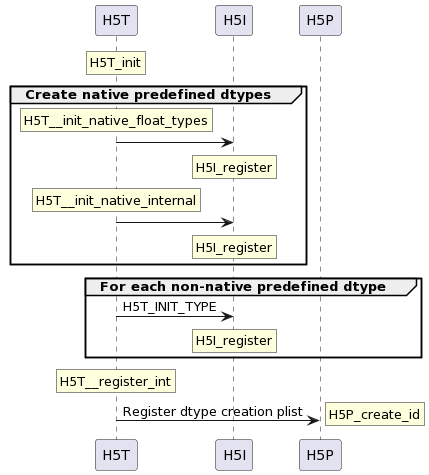
\includegraphics[width=0.55\textwidth]{images/tour_5_uml_h5t_init.png}
\caption{A sequence diagram for \texttt{H5T\_init}}
\label{fig:h5t-init-table}
\end{figure}

\paragraph{User-defined Datatypes} Users may derive their own types from the predefined types by copying them to get a transient, modifiable copy. Figure~\ref{fig:predefined-type-copy} is a minimal example demonstrating user-defined type creation. Figure~\ref{fig:tour-5-uml-datatype-copy} shows the internal operation of \texttt{H5Tcopy}.

\begin{figure}
\centering
\caption{Creation of a user-defined type identical to a platform-native integer.}
\label{fig:predefined-type-copy}
\begin{minted}[linenos]{C}
int main(void) {
    hid_t type_id = H5Tcopy(H5T_NATIVE_INT);
    H5Tclose(type_id);
};

\end{minted}
\end{figure} 

\begin{comment}
http://www.plantuml.com/plantuml/uml/
@startuml
participant H5T
participant "H5T Private" as private
participant H5O
participant H5I

rnote over H5T: H5Tcopy
H5T -> private: H5T_copy (Transient)
rnote over private: H5T__initiate_copy
rnote over private: H5T__complete_copy

H5T -> H5I: Register newly opened datatype object with the library
rnote over H5I: H5I_register()
H5I -> H5T: Datatype handle ID
@enduml
\end{comment}

\begin{figure}
    \centering
    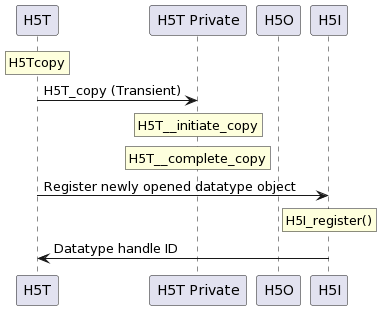
\includegraphics[width=0.5\textwidth]{images/tour_5_uml_datatype_copy.png}
    \caption{H5Tcopy sequence diagram}
    \label{fig:tour-5-uml-datatype-copy}
\end{figure}

\texttt{H5Tcopy} performs the datatype copy operation in two steps. First, \texttt{H5T\_\_initiate\_copy} allocates in-memory structures for the new object and, if the original datatype is committed, increases its in-memory reference count. Then \texttt{H5T\_\_complete\_copy} copies the information for the new datatype from the old datatype. Lastly, \texttt{H5I\_register} assigns a handle ID to the new datatype.

\begin{listing}
\centering
\caption{Committing a type as an HDF5 Object in storage}
\label{lst:type-commit}
\begin{minted}[linenos]{C}
int main(void) {
    hid_t file_id = H5Fcreate("type_test.h5", H5F_ACC_TRUNC, H5P_DEFAULTx2);
    hid_t type_id = H5Tcopy(H5T_NATIVE_INT);
    
    H5Tcommit(file_id, "user_defined_integer", type_id, H5P_DEFAULTx3);

    H5Tclose(type_id);
    H5Fclose(file_id);
};

\end{minted}
\end{listing}

\begin{comment}
http://www.plantuml.com/plantuml/uml/
@startuml
participant H5T
participant H5L

rnote over H5T: H5Tcommit
rnote over H5T: (...)

rnote over H5T: H5T_copy
H5T -> H5L: H5T__commit_named
rnote over H5L: H5L_link_object

rnote over H5T: New committed type object \nis attached to original H5T_t
@enduml
\end{comment}

\begin{figure}
\centering
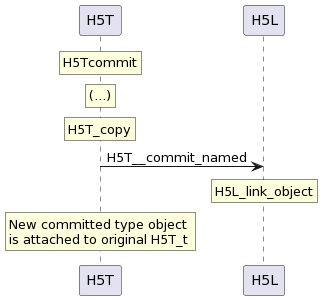
\includegraphics[width=0.4\textwidth]{images/tour_5_uml_datatype_commit.png}
\caption{Internal operation of H5Tcommit}
\label{fig:tour-5-uml-datatype-commit}
\end{figure}

\paragraph{Committed Datatypes} There are two kinds of datatypes: transient datatypes that exist only in memory and committed (formerly "named") datatype objects that are written to storage.

Listing~\ref{lst:type-commit} shows a minimal program that turns a transient datatype into a committed datatype via \\ \texttt{H5Tcommit}. After data is written to the file, the datatype will exist as an object on the file in storage.

Figure~\ref{fig:tour-5-uml-datatype-commit} shows the internal work done by \texttt{H5Tcommit} when using the native VOL. A copy of the provided datatype is created by \texttt{H5T\_copy}, and this copy is written to storage. \texttt{H5T\_\_commit\_named} sets up creation information for \texttt{H5L\_link\_object}, which creates the committed datatype object and a hard link used to link it into the file hierarchy. Lastly, the newly committed datatype object is attached, as an \texttt{H5VL\_object\_t} instance, to the \texttt{vol\_obj} field of the original datatype provided to \texttt{H5Tcommit}.

\subsection{Datatype conversion}\label{sec:dtype-conv}

In this section, we describe the circumstances in which and where datatype conversion takes place during user data transfer and how the library locates appropriate datatype conversion functions at run-time.

\paragraph{Overview} Datatype conversion is performed at transfer (read or write) time. Which conversions are possible depends on the set of defined conversion functions. As a rule of thumb, conversion is possible if the datatypes of the source and destination are different types within the same datatype class. For example, integers can generally be converted to other integers and floats to other floats. Some other common conversions, like integer-to-float and vice versa, are also predefined.

\paragraph{Conversion Functions} Conversion between a source and destination type is performed via a conversion function. A conversion function may be 'hard' or 'soft'. Hard conversion functions are each associated with a particular source and destination datatype, while soft conversion functions are related to entire datatype classes. 

The library maintains a global table of type conversion functions, \texttt{H5T\_g}. Each conversion function is uniquely identified by a ``path'' (\texttt{H5T\_path\_t}) formed from the source and destination datatypes. When a conversion is necessary, a binary search is performed on this table to locate an appropriate conversion function. 

\paragraph{User-Defined Conversion Functions} Users can add new conversion functions or overwrite the behavior of existing conversion functions through \texttt{H5Tregister}. A new hard conversion function will overwrite any previous conversion functions for the specified types, and a new soft conversion function will overwrite the conversion functions for any types to which it is applicable that do not already have a hard conversion function.

\begin{listing}
\centering
\caption{User-defined datatype conversion -- setup.}
\label{lst:ud-datatype-conversion-setup}
\begin{minted}[linenos]{C}
#include "common.h"

typedef struct src_t {
     uint32_t a;
     float b;
  } src_t;

typedef struct dst_t {
     float b;
  } dst_t;

herr_t convert(hid_t src_id, hid_t dst_id, H5T_cdata_t *cdata,
    size_t nelmts, size_t buf_stride, size_t bkg_stride, void *buf,
    void *bkg, hid_t dxpl)
{
  herr_t retval = EXIT_SUCCESS;
  switch (cdata->command)
  {
  case H5T_CONV_INIT:
    printf("Initializing conversion function...\n");
    break;
  case H5T_CONV_CONV:
    printf("Converting...\n");
    for (size_t i = 0; i < nelmts; ++i)
      ((dst_t*) buf)[i].b = ((src_t*) buf)[i].b;
    break;
  case H5T_CONV_FREE:
    printf("Finalizing conversion function...\n");
    break;
  default:
    break;
  }
  return retval;
}
\end{minted}
\end{listing}

Listing~\ref{lst:ud-datatype-conversion-setup} shows a user-defined conversion function \texttt{convert}, which converts between the user-defined compound datatypes \texttt{src\_t} and \texttt{dst\_t}. Notice that the conversion operation, \texttt{H5T\_CONV\_CONV}, occurs entirely within the main buffer. This is straightforward in this case because \texttt{src\_t} is larger than \texttt{dst\_t}, and so the assignment to \texttt{((dst\_t*) buf)[i].b} will never overwrite any memory needing to be read to convert a subsequent element. More complex conversions may need to use the 'background buffer', \texttt{bkg}, as a place for temporary storage.

\begin{listing}
\centering
\caption{User-defined datatype conversion -- invoked directly.}
\label{lst:ud-datatype-conversion-direct}
\begin{minted}[linenos]{C}
int main() {
  hid_t src = H5Tcreate(H5T_COMPOUND, sizeof(struct src_t));
  H5Tinsert(src, "a", HOFFSET(struct src_t, a), H5T_NATIVE_UINT32);
  H5Tinsert(src, "b", HOFFSET(struct src_t, b), H5T_NATIVE_FLOAT);
  hid_t dst = H5Tcreate(H5T_COMPOUND, sizeof(struct dst_t));
  H5Tinsert(dst, "b", HOFFSET(struct dst_t, b), H5T_IEEE_F32LE);
  H5Tregister(H5T_PERS_SOFT, "src_t->dst_t", src, dst, &convert);
  struct src_t buf[] = {
    {1, 1.0} , {2, 2.0}, {3, 3.0}, {4, 4.0} , {5, 5.0} };  
  H5Tconvert(src, dst, 5, buf, NULL, H5P_DEFAULT);
  
  H5Tunregister(H5T_PERS_SOFT, "src_t->dst_t", src, dst, &convert); 
  H5Tclose(dst);
  H5Tclose(src);
  return 0;
}
\end{minted}
\end{listing}

\begin{listing}
\centering
\caption{User-defined datatype conversion -- invoked implicitly during write.}
\label{lst:ud-datatype-conversion-implicit}
\begin{minted}[linenos]{C}
#include "common.h"
herr_t convert_float(hid_t src_id, hid_t dst_id, H5T_cdata_t *cdata,
    size_t nelmts, size_t buf_stride, size_t bkg_stride, void *buf,
    void *bkg, hid_t dxpl)
{
  herr_t retval = EXIT_SUCCESS;
  switch (cdata->command)
  {
  case H5T_CONV_INIT:
    printf("Initializing float conversion function...\n");
    break;
  case H5T_CONV_CONV:
    printf("Converting floats...\n");
    for (size_t i = 0; i < nelmts; ++i)
      ((float*) buf)[i] = ((double*) buf)[i];
    break;
  case H5T_CONV_FREE:
    printf("Finalizing float conversion function...\n");
    break;
  default:
    break;
  }
  return retval;
}

int main() {
  hid_t src = H5Tcopy(H5T_NATIVE_DOUBLE);
  hid_t dst = H5Tcopy(H5T_NATIVE_FLOAT);
  H5Tregister(H5T_PERS_SOFT, "double->float", src, dst, &convert_float);
  double buf[] = {1.0, 2.0, 3.0, 4.0, 5.0};  
  
  hid_t file_id = H5Fcreate("float_conv.h5", H5F_ACC_TRUNC, H5P_DEFAULTx2);
  hid_t space_id = H5Screate_simple(1, (const hsize_t[]) {5}, NULL);
  hid_t dset_id = H5Dcreate(file_id, "dset", dst, space_id, H5P_DEFAULTx3);
  H5Dwrite(dset_id, src, space_id, H5S_ALL, H5P_DEFAULT, buf);
  H5Tunregister(H5T_PERS_SOFT, "double->float", src, dst, &convert_float);
  H5Fclose(file_id);
  H5Dclose(dset_id);
  H5Tclose(dst);
  H5Tclose(src);
  return 0;
}
\end{minted}
\end{listing}

\begin{comment}
http://www.plantuml.com/plantuml/uml/
@startuml
participant H5T 
participant H5D

rnote over H5D: H5Dwrite
rnote over H5D: H5D__write
group Initialize type info for transfer
rnote over H5D: H5D__typeinfo_init
rnote over H5D: H5D__typeinfo_init_phase2
rnote over H5D: H5D__typeinfo_init_phase3
end
rnote over H5D: H5D__contig_write
H5D -> H5T: H5D__scatgath_write
rnote over H5T: H5T_convert
rnote over H5T: User conversion callback
@enduml
\end{comment}

\begin{figure}
    \centering
    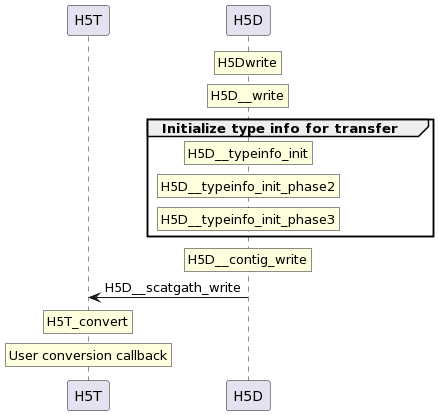
\includegraphics[width=0.50\textwidth]{images/tour_5_uml_datatype_conversion.png}
    \caption{Datatype conversion with user callback diagram}
    \label{fig:tour-5-uml-datatype-conversion}
\end{figure}

Listing~\ref{lst:ud-datatype-conversion-direct} creates compound datatypes corresponding to \texttt{src\_t} and \texttt{dst\_t}, and registers \texttt{convert} as a soft conversion function from\texttt{src} to \texttt{dst}. It invokes the library's top-level conversion function \texttt{H5Tconvert}, automatically finding the newly registered conversion function by a path. 

Datatype conversion can also be done automatically by the library during writes or reads. Listing~\ref{lst:ud-datatype-conversion-implicit} shows an example of a program where a user-defined conversion between floats is done automatically during a write to a dataset. 

Figure~\ref{fig:tour-5-uml-datatype-conversion} illustrates how type conversion happens during a write to a dataset. The library's internal dataset write function \texttt{H5D\_\_write} initializes datatype information in three phases. The initialization is done in phases due to requirements imposed by parallel I/O. Specifically, when doing parallel I/O, the maximum datatype size across all destination objects must be computed after the first phase, and the selection in the destination datasets must be adjusted after the second phase. 

The first phase of type info initialization, \texttt{H5D\_typeinfo\_init}, populates the \texttt{type\_info} field of each dataset's \texttt{H5D\_dset\_io\_info\_t} structure with the appropriate datatype conversion function, the size of each datatype, and whether this is the special case of converting between compound datatypes that are subsets of one another. Unlike the other phases, the first phase is done separately for each destination dataset. 

The second phase, \texttt{H5D\_\_typeinfo\_init\_phase2}, checks if selection I/O can be used and if the (expected) size of the conversion buffer and background buffer are sufficient to perform the conversion with the given selection. 

The third and final phase, \texttt{H5D\_\_typeinfo\_init\_phase3}, allocates a type conversion buffer and a background buffer of appropriate size for each dataset that requires them and did not have them provided through transfer properties.

After the type info for the transfer is fully initialized, the write proceeds through a write callback specific to the layout of the target dataset(s). For example, for the program in Listing~\ref{lst:ud-datatype-conversion-implicit}, the dataset's layout is \texttt{H5D\_CONTIGUOUS}, and so the write callback is \texttt{H5D\_\_contig\_write}. To gather elements from the user-provided buffer for contiguous writes to disk, \texttt{H5D\_\_scatgath\_write} is invoked. Type conversion is then performed in the provided buffers right before the data is scattered to the file. 


\subsection{Datatype metadata \& value encodings}


In this section, we describe the datatype metadata retained in the HDF5 library and files, how the values of certain non-fixed-size datatypes are represented and encoded, and how the datatype affects where encoded values are stored in the HDF5 file.

\paragraph{Overview of Datatype Metadata Storage} An HDF5 file is stored on disk as a global heap and data objects (among other things outside the scope of this section). Each data object has an 'object header' and 'object information.' The object information is the user's stored data, e.g., scientific measurements. The object header contains 'messages' which describe metadata regarding the information object. 

Datatypes exist on disk as Datatype Messages according to the HDF file format. A Datatype Message contains information about the datatype's size, class, and class-specific properties.

Transient datatypes are not written to disk unless they are used to create attributes or datasets. In this case, the object header for the attribute or dataset will contain a Datatype Message describing the datatype.

Recall that committed datatypes must be linked into the file hierarchy. A committed datatype is stored on disk as an object header with a Datatype Message. If a committed datatype is used in a dataset or an attribute, then the Datatype Message for that dataset or attribute contains a pointer to the original committed datatype's Datatype Message - the information is not duplicated.


% \paragraph{Datatype Metadata} A file retains the metadata about a datatype necessary to reconstruct it when reading from the file. The first 8 bytes of a Datatype Message describe the class of the datatype, the size of an instance of the datatype, and some class-specific flags. Because 4 bytes (32 bits) in the message are for the size of a datatype instance, a single element in a dataset or attribute cannot be larger than $2^{32} -1 \approx $ 4 gigabytes. After the first 8 bytes of the message is a properties section without a fixed length, which contains information specific to each datatype class. The specifics of these properties are detailed in the file format documentation.

\paragraph{Datatype Encoding} Datatype encoding is the process of converting an in-memory datatype object (\texttt{H5T\_t}) to a series of bytes which may be written to storage as a Datatype Message. This process may be invoked explicitly by \texttt{H5Tencode/H5Tdecode} or implicitly when writing objects with a datatype to storage. 

Figure~\ref{fig:tour-5-uml-datatype-encode} shows the library's datatype encodeing process. Some internal routines require a valid \texttt{H5F\_t} file struct but do not modify or depend on a real external file. To support datatype encoding/decoding without a real associated file, \texttt{H5F\_fake\_alloc} creates a 'fake' file struct with no counterpart in storage. The size of the message to create is determined by \texttt{H5O\_msg\_raw\_size}, which invokes the Datatype Message class's  'size' callback, \texttt{H5O\_\_dtype\_size}. Similarly. the generic \texttt{H5O\_msg\_encode} invokes the Datatype Message class's encode callback, \texttt{H5O\_\_dtype\_encode}. This encode callback populates the provided buffer with information from the datatype. Suppose the datatype is non-atomic; recursive calls to \texttt{H5O\_\_dtype\_encode\_helper} populate each component datatype. For compound types, a separate recursive call encodes each member field. A single recursive call is used to encode the base type for arrays, variable-length types, and enums.

\begin{comment}
http://www.plantuml.com/plantuml/
@startuml
rnote over H5T: H5Tencode
rnote over H5T: H5T_encode

H5T -> H5F: Get fake file struct
rnote over H5F: H5F_fake_alloc

H5T -> H5O: Compute msg size
rnote over H5O: H5O_msg_raw_size
rnote over H5O: H5O__dtype_size

H5T -> H5O: Encode dtype to msg recursively
rnote over H5O: H5O_msg_encode
rnote over H5O: H5O__dtype_encode
rnote over H5O: H5O__dtype_encode_helper

opt Non-atomic dtype
rnote over H5O: Recursive call(s)
rnote over H5O: H5O__dtype_encode_helper
end
@enduml
\end{comment}

\begin{figure}
    \centering
    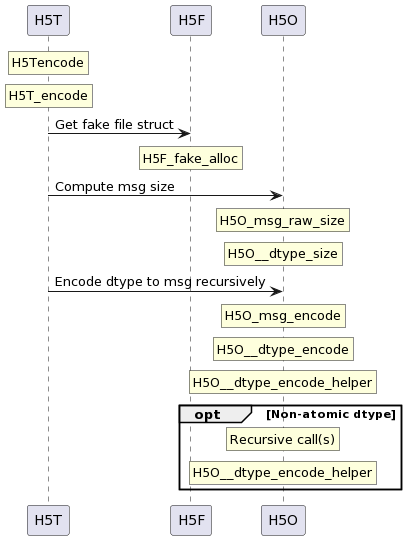
\includegraphics[width=0.45\textwidth]{images/tour_5_uml_datatype_encode.png}
    \caption{Datatype encoding process}
    \label{fig:tour-5-uml-datatype-encode}
\end{figure}

\paragraph{Datatype storage} Data with a simple atomic datatype is stored in the object information section of the data object. Because elements of more complex datatypes may have an indeterminate or variable size, they must be stored differently. Variable-length and region reference data are stored in the file's global heap. Object reference data is stored as the offsets necessary to read from the object header of the referenced object. Compound datatype elements are stored as a contiguous stream of the structure's items, each formatted according to its datatype.

\subsection{Summary} 

In this tour, we covered the different categories of datatypes, how they are represented and handled by the library, and how objects use them. We reviewed how datatypes are encoded for storage on disk and how data of different datatypes is stored in the file.

The ability for the user to define their own datatypes, composite datatypes, and datatype conversion functions is another example of the extensibility and customizability of the HDF5 library, allowing users to optimize nearly every step in the I/O process.